 
% rtlu.factor
 	\begin{center}
	\addtolength{\leftskip}{-4cm}\addtolength{\rightskip}{-4cm}

\begin{tabular}{|c|c|}
\hline
\multicolumn{2}{|c|}{\textbf{\underline{\textbf{\underline{data$nativeTown}}}}}\\

\multicolumn{2}{|c|}{Nominal(12) \hfill N=156 ; NA=16 (10.26\%)}\\
\hline
 \textbf{Frequency} & \textbf{Histogram} \\

 \begin{tabular}{@{}l@{ : }cl@{}}

  Autre & 54 & (38.57\%) \\

  Paris & 34 & (24.29\%) \\

  Saint Germain en Laye & 9 & (6.43\%) \\

  Suresnes & 9 & (6.43\%) \\

  Courbevoie & 8 & (5.71\%) \\

  Colombes & 7 & (5\%) \\

  Neuilly & 5 & (3.57\%) \\

  Nanterre & 4 & (2.86\%) \\

  Poissy & 4 & (2.86\%) \\

  Argenteuil & 2 & (1.43\%) \\

  Boulogne Billancourt & 2 & (1.43\%) \\

  Garenne Colombes & 2 & (1.43\%) \\

 \end{tabular}
 & \parbox{13cm}{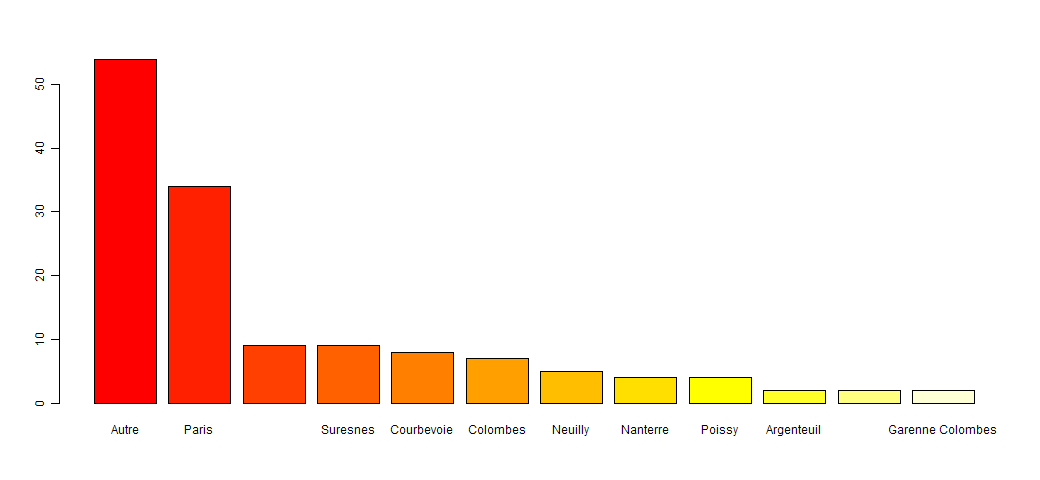
\includegraphics[width=13cm]{graphUniv3/V-barplot.png}}
 \\
\hline
\end{tabular}
\end{center} 
